\section{Introduction}

Attitude estimation is an essential task in robotics. There is a ground robot that capable of high maneuverability by freely tilting its upper body as shown in Fig.\ref{fig:CCV}. In such robots, a failure of the attitude estimation has serious consequences, such as falls. Usually, robots use sensors such as IMU to estimate their attitude. However, in the case of ground robots, drift and bias due to unevenness and slippage of the ground can make attitude estimation difficult\cite{Vaganay1993MobileRA}. This means that the estimation of the attitude by relying on the internal sensor is difficult.

   \begin{figure}[thpb]
      \centering
      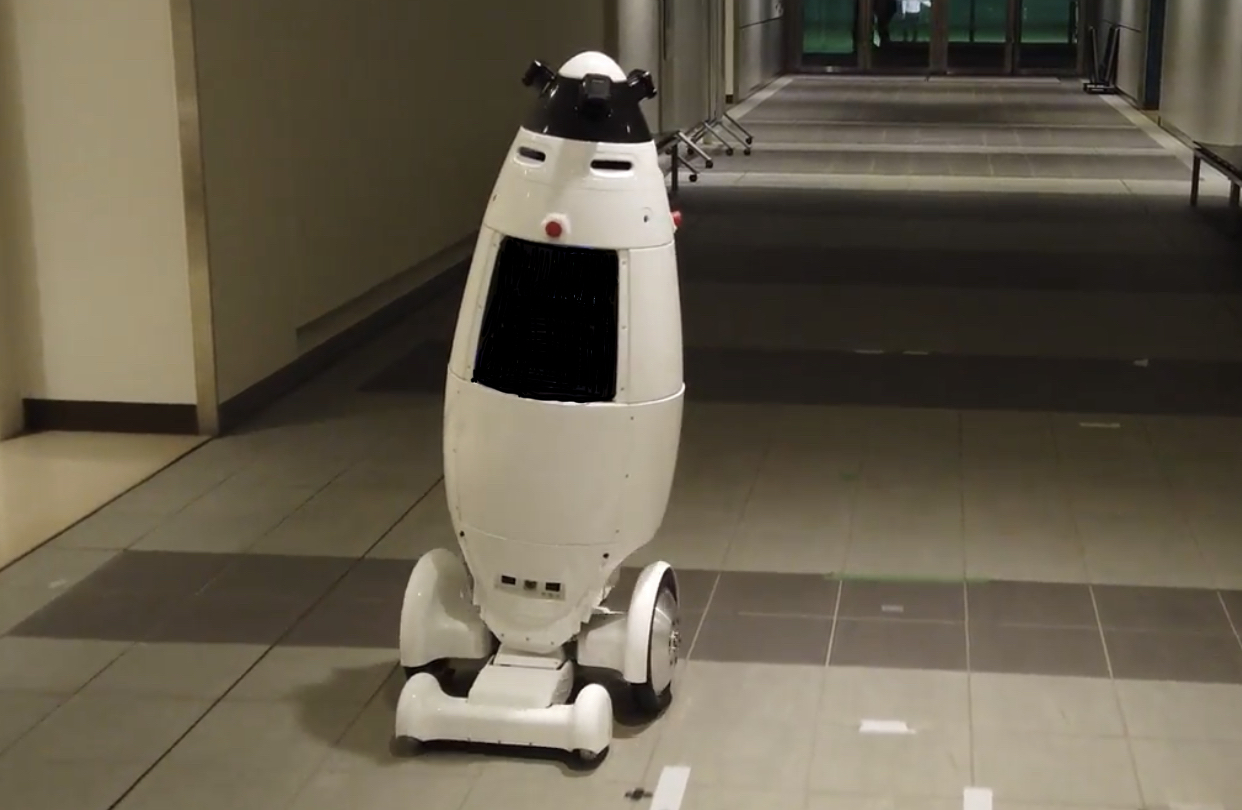
\includegraphics[scale=0.13]{./figure/1_introduction/CCV.jpg}
      \caption{Robots can perform high maneuverability by freely
tilting their upper body}
      \label{fig:CCV}
   \end{figure}

To address this problem, there are much research on attitude estimation using SLAM techniques\cite{thrun2005probabilistic}. However, SLAM is associated with problems such as failure due to dynamic obstacles\cite{SLAM_fail} and high computational cost. This type of method has a problem of error accumulation. This causes significant problems when operating long distances or for long periods. Therefore, there is a need for robots to perform attitude estimation without error accumulation. \par
   
 \begin{figure*}[!t]
    \centering
    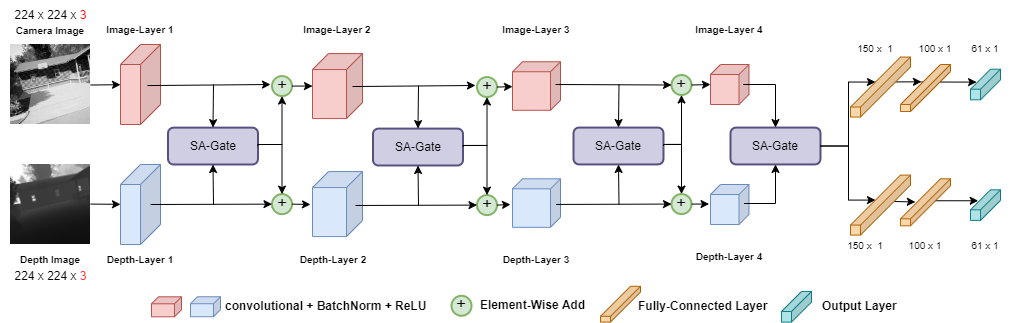
\includegraphics[scale=0.38]{./figure/2_method/SII2023_network_overall_2.png}
    \caption{Network Architecture. The training and test images were grayscaled to compress data size and speed up processing. However, when inference is used, the number of channels is 3 to make it a pre-trained ResNet input.}
    \label{fig:network_overall}
\end{figure*}

 \begin{figure*}[!t]
    \centering
    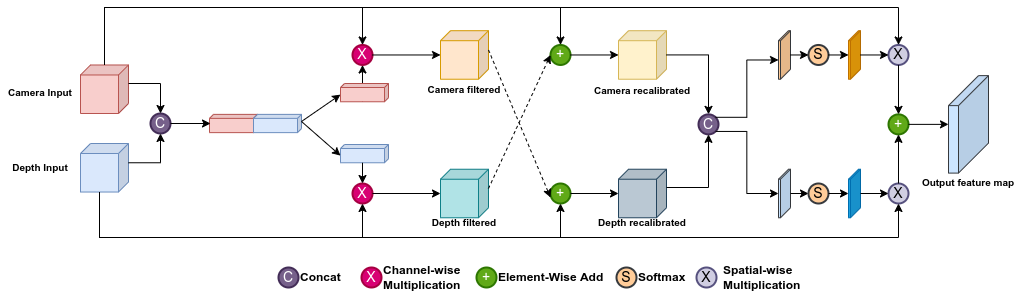
\includegraphics[scale=0.38]{./figure/2_method/sa_gate.png}
    \caption{SA-Gate Architecture}
    \label{fig:sagate_overall}
\end{figure*}

Ozaki proposed an attitude estimation method by extracting normal vectors from point clouds from LiDAR scan and integrating information from gyroscope and wheel odometry, based on the assumption that walls are mostly vertical to the horizontal plane in environments with artificial objects such as inside buildings\cite{ozaki_lidar_normal}. However, this approach is based on the assumption that there were many buildings and other human-made structures in the surrounding area. To solve this problem, he proposed a method to estimate the attitude using camera image and deep learning\cite{Ozaki_SII2021}. This method enables non-rule-based attitude estimation by training a numerical regression neural network with attitude data associated with camera images. Other methods exist to estimate the attitude by integrating the information from the gyroscope with the inference from the camera image using a numerical regression neural network\cite{ozaki_springer}. Attitude estimation from camera images using DNN, as in these methods, has the advantage of eliminating error accumulation. However, when the output layer is used as a numerical regression, the accuracy of the estimation is insufficient. This is due to the small number of parameters near the output layer, and the inadequacy of the expressive power of the numerical regression compared to the capability required for the attitude estimation task.

%尾崎は建物内などの人工物のある環境下では壁は水平面に対して鉛直であることがほとんどであるという前提のもと、LiDARから得られる点群から法線ベクトルを抽出、ジャイロスコープとホイールオドメトリからの情報を統合することでの姿勢推定手法を提案した。しかし、この手法は建物などの人工物が周囲に多数存在していることが前提であった。翌年彼は姿勢をカメラからの画像を深層学習を用いて推定する手法を提案した。この手法はカメラ画像と紐付けた姿勢のデータを数値回帰型のニューラルネットワークに学習させることでルールベースによらない姿勢推定を可能にするとともに、Monte-Carlo dropoutを用いることで深層学習の不確かさを推定することも可能にした。これらの手法のように、カメラ画像からDNNを用いてattitude estimationを行うことはerror accumulationがないといったメリットがある。しかし、output layerをnumerical regressionにした場合、estimationの精度は不十分であった。これはoutput layer付近のパラメータ数が少ないことが原因で、numerical regressionの持つ表現能力がattitude estimation taskに求められる能力に対して不十分であったことが原因であると考えられる

In our previous work, we achieved high attitude estimation accuracy by introducing a classification type output layer to neural network\cite{9708864} based on OCR method. But this method still has a problem with estimation accuracy in an unknown environment. To put camera attitude estimation using deep neural networks into practical use for a ground robot, it is necessary to improve the accuracy of attitude estimation in unknown environments. The key elements for this are a prior knowledge that the wall is vertical to the ground and the ground is horizontal, which played a key role in Ozaki's study\cite{ozaki_lidar_normal}, and sensors that can obtain this information. In this paper, the depth camera was adopted as a tool to obtain topographic information. Terrain information can also be obtained from LiDAR. However, the form of data obtained from LiDAR is very different from that of RGB images, making it a hard task to use as input for DNN\cite{ozaki_robosym}. In DNN, the integration of information from LiDAR and from the camera alone is a valid research project\cite{google_LiDAR_camera}. On the other hand, the depth image can be sampled with the same position, viewing angle, and size as the Image camera using equipment, enabling feature extraction where information from the camera image and information from the depth image interfere with each other.

%deep neural networkによるcamera attitude estimationを実用化するためにはunknown environmentでのattitude estimationの精度を向上する必要がある。これのために重要となる要素がOzakiのstudyでも重要な役割を果たした、壁は地面に対して垂直、地面は水平であるなどの事前知識と、それを情報として入手できるセンサである。地形の情報はLiDARからも入手することができる。しかし、LiDARは得られるデータの形態がRGB画像とは大きくかけ離れており、DNNのinputとするのには不適である。DNNにおいては、LiDARからの情報とカメラからの情報の統合だけでも一つの研究として成立する。その一方で、depth画像はIntel Realsenseなどの機器を用いればRGBカメラと同一の位置や視野角、サイズを持って画像を採取することが可能であり、RGB画像からの情報とdepth画像からの情報を相互に干渉し合う特徴量抽出を可能とする。

Feature extraction methods that intermingle information from camera and depth images have been used successfully in the field of semantic segmentation\cite{DBLP:journals/corr/abs-2011-06961}. These methods add information from the depth image as a supplement to the usual semantic segmentation. But Chen et al proposed a feature extraction method\cite{SAGATE} that interferes with information from the HHA image generated from the depth image and the camera image to improve segmentation accuracy and ensure the robustness of feature extraction. In this paper, to improve the accuracy of attitude estimation in unknown environments, the feature extraction module used in the method of Xing et al. is employed in the attitude estimation network. \par


%RGB画像とdepth画像、この2つから得られる情報を相互に干渉させながら特徴量抽出を行う手法はsemantic segmentationの分野で成功を収めている。これらの手法は通常のsemantic segmentationにdepth画像の情報を補助として加えるものであったが、Xingらはdepth画像から生成されるHHA画像とRGB画像からの情報を相互に干渉させて特徴量抽出を行う手法を提案し、segmentationの精度向上と特徴量抽出のロバスト性の確保を達成した。この論文では、未知環境での姿勢推定精度向上のために、Xingらの手法で用いられている特徴量抽出モジュールをattitude estimation networkに採用する

In this paper, we aim to improve the accuracy of attitude estimation in unknown environments by using different types of images as inputs: camera images for scenery and depth images for terrain information. The main contributions of this paper are as follows

%この論文では、風景画像を得られるcamera imageと地形情報を得られるdepth imageの異なる種類を持つ画像をinputとして、unknown環境におけるattitude estimationの精度改善を狙う。

\begin{itemize}
\item Highly accurate attitude estimation by introducing a feature extractor that can extract both topographic and landscape information.
\item Improved accuracy of attitude estimation in unknown environments in simulators.
\item Effectiveness of the classification type output layer in the task of estimating the attitude.
\end{itemize}